\documentclass[final]{beamer}

% ====================
% Packages
% ====================
\usepackage{fontenc}
\usepackage{lmodern} % Load modern fonts
\usepackage[orientation=portrait,size=a3,scale=1.15]{beamerposter}
\usetheme{gemini}
\usecolortheme{nott}
\usepackage{graphicx}
\usepackage{booktabs}
\usepackage{tikz}
\usepackage{pgfplots}
\usepackage{chemfig}
\usepackage{mhchem}
\pgfplotsset{compat=1.14}
\usepackage{anyfontsize}

% ====================
% Lengths
% ====================
\newlength{\sepwidth}
\newlength{\colwidth}
\setlength{\sepwidth}{0.025\paperwidth}
\setlength{\colwidth}{0.45\paperwidth}

\newcommand{\separatorcolumn}{\begin{column}{\sepwidth}\end{column}}

% ====================
% Title
% ====================
\title{\vphantom{Hvordan fører \text{\textit{Tetraetylbly (\ce{Pb(C_2H_5)_4})}} til kognitiv svekkelse?}}
\author{\vphantom{Temor Yari}}
\institute[Bjerke Videregående Skole]{\vphantom{Bjerke Videregående Skole}}

% ====================
% Footer (optional)
% ====================
\footercontent{2}

% ====================
% Logo (optional)
% ====================
% use this to include logos on the left and/or right side of the header:
% \logoright{\includegraphics[height=2.5cm]{logos/utfpr-logo.png}}
% \logoleft{\hspace{20ex}\includegraphics[height=3.5cm]{logos/ppgca-logo.png}}

% ====================
% Body
% ====================
\begin{document}

\begin{frame}[t] % Second paper
	\begin{columns}[t]
		\separatorcolumn

		\begin{column}{\colwidth}

			\begin{alertblock}{Resultat}
				Akkumulering av \textbf{\delta-aminolevulinsyre (ALA)} i hjernen som følge av blyforgiftning
				utløser en kaskade av skadelige prosesser med alvorlige konsekvenser for kognitiv funksjon.
				ALA gjennomgår auto-oksidasjon og genererer reaktive oksygenforbindelser (ROS) som
				\textbf{skader nevronale strukturer}. Samtidig påvirker bly og ALA-deriverte radikaler
				nøkkelproteiner som \textit{Calmodulin} og \textit{proteinkinase C (PKC)}, som er avgjørende
				for \textit{synaptisk plastisitet}, læring. Forskning viser en konsistent \textbf{invers
					sammenheng} mellom blynivåer i blodet og \textbf{IQ}, der hver \textbf{\textit{10 μg/dL}}
				økning i blodnivåer hos barn medfører en gjennomsnittlig nedgang på \textbf{\textit{2-5
						IQ-poeng}} . Denne relasjonen følger en ikke-lineær kurve der selv lave blynivåer har
				betydelig effekt, noe som indikerer at det ikke finnes en trygg nivå for blyeksponering,
				særlig hos barn med utviklende nervesystem.

				\begin{figure}[h!]
					\centering
					\vspace{0.5cm}
					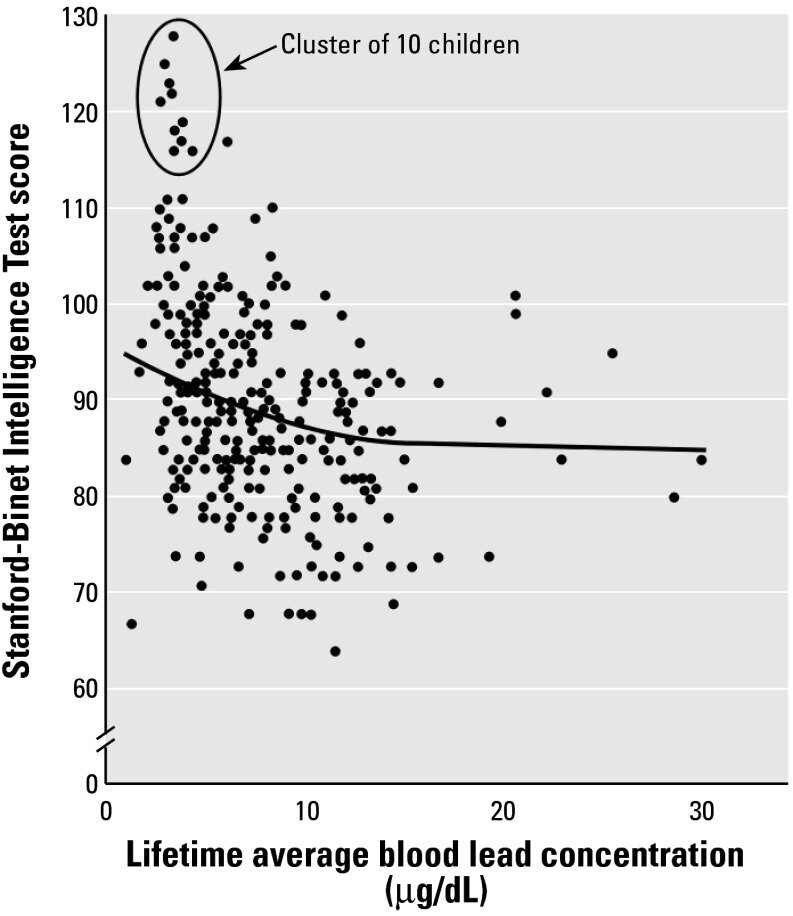
\includegraphics[width=10cm]{./assets/IQ_lead_relation.jpg}
					\caption{Forholdet mellom avg. bly in blodet og IQ}
				\end{figure}
			\end{alertblock}



			\begin{block}{Clair Patterson og utfasning av Bly}
				Utfasing av blyholdig bensin ble drevet av flere viktige vitenskapelige funn.
				\textbf{Geokjemikeren Clair Patterson} påviste at blyforurensning i miljøet var
				\textbf{menneskeskapt} ved å analysere isotopforhold i blyprøver. \textbf{Herbert Needleman}
				avdekket en sammenheng mellom blyeksponering og kognitive svekkelser hos barn, der høyere
				blynivåer i tenner korrelerte med lavere IQ og redusert oppmerksomhet. Videre viste
				luftprøver fra iskjerner at atmosfærisk blytransport økte i takt med global bruk av
				blyholdig bensin, noe som understreket den omfattende spredningen av blyforurensning.

				\begin{figure}[h!]
					\centering
					\vspace{0.5cm}
					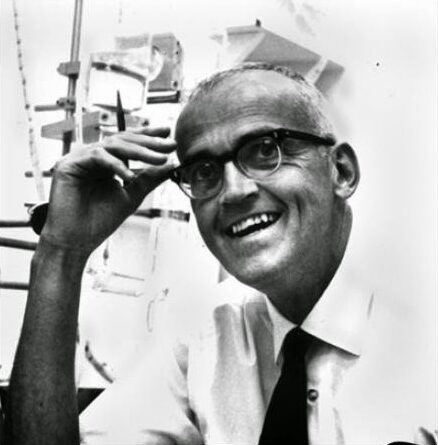
\includegraphics[width=10cm]{./assets/clair-patterson.jpg}
					\caption{Geokjemikeren Clair Patterson}
				\end{figure}

			\end{block}
		\end{column}

		\separatorcolumn

		\begin{column}{\colwidth}

			\begin{block}{Reguleringer og utfasningsstrategier}
				Vitenskapelige bevis førte til regulatoriske tiltak verden over. \textbf{USA} startet en
				gradvis reduksjon av blyinnholdet i bensin i 1975, med full forbud i \textbf{1996}.
				\textbf{EU} innførte lignende tiltak, som sikret et totalforbud innen \textbf{2000}. På
				globalt nivå tok \textbf{FN} gjennom UNEP initiativ til en internasjonal utfasingsplan i
				2002. Mens 82 land fortsatt brukte blyholdig bensin på den tiden, var \textbf{Algerie} det
				siste landet som avviklet bruken i \textbf{2021}, noe som markerte slutten på blyholdig
				bensin globalt.

			\end{block}

			\begin{block}{Alternativer til tetraetylbly}
				For å erstatte tetraetylbly (TEL) ble flere teknologiske alternativer utviklet.
				\textbf{Metyltertiærbutyleter (MTBE)} og \textbf{etanol} ble populære for å øke oktantallet,
				selv om MTBE skapte miljøproblemer. \textbf{Metylcyklopentadienylmangan-trikarbonyl (MMT)}
				tilbød en mindre giftig løsning, mens bensinreformulering gjennom katalytisk reformering og
				isomerisering forbedret drivstoffkvaliteten. I tillegg reduserte \textbf{avanserte
					motorteknologier} som elektronisk tenningskontroll og direkteinnsprøytning behovet for
				blybaserte antiknock-midler.
			\end{block}

			\begin{block}{Ord- og begrepforklaringer}


				\begin{enumerate}

					\item \textbf{Antikloppmiddel}: En substans som hindrer prematur tenning ("banking") i
					      forbrenningsmotorer.
					\item \textbf{Oktantall}: Et mål på et drivstoffs evne til å motstå selvtenning under
					      kompresjon.
					\item \textbf{Organometallisk forbindelse}: En kjemisk forbindelse som inneholder minst én
					      direkte binding mellom karbon og et metall.
					\item \textbf{Reaktive oksygenspecies (ROS)}: Kjemisk reaktive forbindelser som inneholder
					      oksygen, som kan skade cellulære komponenter.
					\item \textbf{Sulfhydrylgruppe (-SH)}: En funksjonell gruppe bestående av svovel og
					      hydrogen, som finnes i aminosyren cystein.
					\item \textbf{Oksidativt stress}: En ubalanse mellom produksjon av frie radikaler og
					      kroppens evne til å nøytralisere dem.
					\item \textbf{Etylradikal (\textbullet\ce{C_{2}H_{5}})}: Et ustabilt molekyl med et uparet
					      elektron, dannet gjennom homolytisk kløving av en kjemisk binding.
					\item \textbf{Blod-hjerne-barriere}: Et selektivt permeabelt grensesnitt som separerer
					      blodsirkulasjonen fra ekstracellulærvæsken i sentralnervesystemet.
					\item \textbf{Hemoglobin}: Et jernholdig protein i røde blodceller som transporterer
					      oksygen fra lungene til kroppens vev.
					\item \textbf{Synaptisk plastisitet}: Evnen til synapser til å styrkes eller svekkes over
					      tid, som respons på økt eller redusert aktivitet.
					\item \textbf{Bioakkumulering}: Prosessen der kjemikalier akkumuleres i organismen over
					      tid, ofte i fettvev.
					\item \textbf{Metylcyklopentadienylmangan-trikarbonyl (MMT)}: En organometallisk
					      mangankompleks som brukes som antikloppmiddel.
					\item \textbf{Metyltertiærbutyleter (MTBE)}: En organisk forbindelse som brukes som
					      bensintilsetning for å øke oktantallet.
				\end{enumerate}
			\end{block}

			\begin{block}{Kilder og Referanser}

				\nocite{*}
				\footnotesize{\bibliographystyle{plain}\bibliography{poster}}

			\end{block}

		\end{column}
		\separatorcolumn

	\end{columns}
\end{frame}
\end{document}
